\documentclass[a4paper,11pt]{article}
 \providecommand{\tightlist}{%
     \setlength{\itemsep}{0pt}\setlength{\parskip}{0pt}}
\usepackage{graphicx}
\usepackage{jheppub} 
\usepackage{comment} 
\usepackage[dvipsnames]{xcolor}
\usepackage{tikz}
\usepackage{slashed}
\usepackage{pgfplots}
\usepackage{booktabs, longtable}
\bibliographystyle{JHEP.bst}

\newcommand{\Shufang}[1]{{\bf\color{Maroon}  #1}}
\newcommand{\Adarsh}[1]{{\bf\color{RoyalBlue} AP: #1}}
\newcommand{\ap}[1]{\textcolor{RoyalBlue}{#1}}
\renewcommand{\H}{\widetilde{H}^0}
\newcommand{\B}{\widetilde{B}^0}
\newcommand{\N}{\widetilde{\chi}^0}
\newcommand{\image}[2]{\parbox{#1\textwidth}{\includegraphics[width=#1\textwidth]{images/#2.pdf}}}
\newcommand{\met}{{\slashed{E}_T}}




\title{Higgs Assisted Razor Search for Higgsinos at 100 TeV}
\author[a]{Adarsh Pyarelal}
\author[b]{and Shufang Su}
\affiliation[a]{School of Information, University of Arizona, Tucson, AZ 85718 , USA}
\affiliation[b]{Department of Physics, University of Arizona, Tucson, AZ 85718, USA}

% e-mail addresses: one for each author, in the same order as the authors
\emailAdd{adarsh@email.arizona.edu}
\emailAdd{shufang@email.arizona.edu}


\abstract{% 
  A 100 TeV proton-proton collider will be an extremely effective 
  way to probe the electroweak sector of the Minimal Supersymmetric 
  Standard Model (MSSM). In this paper, we describe a search strategy  
  for discovering pair-produced Higgsino-like NLSPs  at a 100 TeV 
  hadron collider that decay to Bino-like LSPs via intermediate Z and 
  SM Higgs bosons that in turn decay to a pair of leptons and a pair of 
  $b$-quarks respectively: $\N_{2,3}\N_{3,2}
  \rightarrow (Z\N)(h\N)\rightarrow 
  bbll+\N\N$. In addition, we examine 
  the potential for machine learning techniques to boost the power of 
  our searches. Using this analysis, Higgsinos up to 1.3 TeV can be 
  discovered for Binos  up to 0.9 TeV using 3000 fb$^{-1}$ of data,  
  Additionally, Higgsinos up  to 1.8 TeV can be excluded for Binos up 
  to 1.3 TeV at 95\% C.L. \\
  
  \noindent \Shufang{Abstract need to be more detailed.  Let's worry about this after we
  get the draft done.   } \\
}

\begin{document} 
\maketitle
\flushbottom

\section{Introduction}
 
The existence of dark matter provides unambiguous evidence of new 
physics beyond the Standard Model (SM) of particle physics. Indeed, 
given that there is far more dark matter in the Universe than there 
is baryonic matter, determining its precise nature is one of the most 
exciting challenges in particle physics today.  One promising group 
of candidate for dark matter is the class of stable particles known as 
weakly interacting massive particles (WIMPs). These particles arise 
naturally in many extensions of the SM that are motivated by the need to
stabilize the electroweak scale. One of the most studied extensions
to the SM is the Minimal Supersymmetric Standard Model
(MSSM), which predicts a `supersymmetric partner', or \emph{superpartner}, 
for each SM particle\footnote{For a detailed review of the MSSM, see 
Ref. \citep{Martin:1997ns}.}. In the MSSM with \emph{R}-parity conservation, the 
lightest supersymmetric partner (LSP) is predicted to be absolutely 
stable, making it a good candidate for dark matter. The identity of 
the LSP is determined by the mass hierarchy of the superpartners, 
which in turn depends on how supersymmetry is broken.
However, taking into account experimental constraints and phenomenological 
considerations, the lightest of the  MSSM particles known as the 
neutralinos emerges as the most attractive candidate for the LSP \citep{Bertone:2004pz}. 

% Why go beyond the MSSM?
Though a natural MSSM spectrum has the potential to tame the hierarchy
problem, it is under siege from recent data from the Large Hadron
Collider (LHC) \cite{Aaboud:2018ujj, Sirunyan:2018vjp}. 
A compelling alternative scenario comes in the form of
split supersymmetry (split SUSY) \citep{Wells:2003tf,
ArkaniHamed:2004yi, Giudice:2004tc}. In this scenario, the lightest
superpartners are the fermionic ones, on the
scale of 1-10 TeV, while the scalar superpartners can be much heavier,
on the scale of 100 - 1000 TeV. In exchange for accepting some level of
fine-tuning, we obtain numerous benefits, including the suppression of
flavor-changing neutral currents and greater compatibility with data
from CP-violation experiments.  The low lying 
fermionic superpartners consist of neutralinos and charginos (collectively known as Electroweakinos), and gluinos. The current LHC search limits on gluinos are already around xxx TeV~\cite{}.  The limits on Electroweakinos, howeer, are still relatively weak: around xxx $-$ xxx GeV~\cite{}, depending on the decay modes of the parent electroweakinos.  \Shufang{add ref for gluno limit and electroweakino limits.  Fill in the number.} In this paper, we will focus on the discovery potential of the neutralinos and charginos at the 100 TeV $pp$ collider. 
 



% Point to review papers for enumeration of studies
The decay patterns of the Electroweakinos (Winos, Binos, and Higgsinos)
depend on the hierarchy of the MSSM parameters $M_1, M_2$, and $|\mu|$, which 
roughly determine the masses of the Bino, Winos, and Higgsinos, respectively.
In this paper, we consider the Higgsino NLSP and Bino LSP scenario with $M_1 < |\mu| \ll M_2$.
One of the motivations for studying Higgsinos is that the parameter $\mu$ 
that governs its mass plays an important role in electroweak symmetry breaking 
\citep{Acharya:2014pua}. Finding Higgsinos has traditionally been more challenging 
than finding Winos, due to their lower production rate. This, however, can 
be remedied by the increased  production cross sections and luminosities 
at a 100 TeV collider.


 

Since the Bino is the only supersymmetric particle lighter than the Higgsino in the mass hierarchy we consider, the neutral Higgsino will decay to a Bino and a neutral SM boson (\emph{Z/h}) with a branching ratio of 100\%. 
Search for Higgsinos with intermediate gauge boson and  multi-lepton final states have been studied in Ref.~\cite{Gori:2014oua}. \Shufang{Add more details for that study.  Which channel, search resutls, etc.  This would be our comparison for our analyses.}  In this paper we attempt to exploit the relatively high branching ratio of 
the SM Higgs boson to \emph{b} quarks, and study the decay mode $\chi_2^0\chi_3^0\rightarrow Zh \chi_1^0\chi_1^0\rightarrow bb\ell\ell \met$.

% Why a 100 TeV collider?
A 100 TeV collider would open up an immense number of physics
opportunities not afforded to a 14 TeV collider, including exploring the
most interesting regions of the split SUSY parameter space
\citep{Arkani-Hamed:2015vfh}.
% Status of 100 TeV planning
Such a collider would be a natural next step after the LHC, and is being
actively discussed in the particle physics community, with two major
proposals being the FCC-hh by CERN \citep{FCC-hh}, and the SppC  
in China \citep{CEPC}.  As the next energy frontier machine, it is of 
crucial importance to fully explore the physics potential of a 100 TeV $pp$
collider, especially for new particles that are either too heavy or too rare 
to be produced at the LHC~\citep{Arkani-Hamed:2015vfh,Contino:2016spe,Golling:2016gvc,Mangano:2016jyj}.
In particular, studies have already been performed on the prospects of
discovering neutralino dark matter for compressed \cite{Low:2014cba, diCortona:2014yua,Cirelli:2014dsa,Mahbubani:2018tin,Han:2018wus}
and well-separated \cite{Gori:2014oua,Acharya:2014pua}
neutralino spectra.


We use razor variables~\citep{Rogan:2010kb} in our study, which were originally designed
for searches involving two heavy, mass-degenerate pair-produced
particles, each of which decays into a visible and invisible set of
particles. This topology matches that of our search channel, making this
set of variables a natural choice for our analysis.  

At a 100 TeV collider, the backgrounds are going to be even larger than
at the LHC.  An ancillary goal of this paper is to investigate the
potential for machine learning (ML) techniques to augment our analysis.
With the advent of more powerful computers and simultaneous advances in
the field of statistical learning in recent years, the usage of ML is
rising in experimental particle physics - in fact, the discovery of the
SM Higgs boson in 2012 was done with the help of neural networks
\citep{Aad:2012tfa} and boosted decision trees (BDT)
\citep{Chatrchyan:2012xdj}.

The rest of the paper is structured as follows. In Sec.~\ref{sec:model}, we describe our model and search channel in more
detail, and list the existing experimental constraints on it. In Sec.~\ref{sec:analysis}, we describe our analysis strategies 
for both traditional cut-and-count analyses and analyses
performed using BDT. In Sec.~\ref{sec:results},
we present the results of our analyses, i.e. the expected discovery and exclusion
reaches. Finally, we conclude with the implications in Sec.~\ref{sec:conclusion}.

\section{The neutralino sector of the MSSM}
\label{sec:model}

 
The neutralino sector of MSSM consists of four mass eigenstates
($\N_1,\N_2,\N_3,\N_4$), which
are mixtures of the Bino, Wino, and two neutral Higgsinos: 
($\B,\widetilde{W}^0,\H_u,\H_d$). In the basis of these gauge eigenstates, the mass
matrix of the neutralinos can be written as

\newcommand{\cb}{ c_\beta}
\newcommand{\cw}{ c_W}
\newcommand{\sinb}{ s_\beta}
\newcommand{\sw}{ s_W}
\newcommand{\mz}{ m_Z}

\[\mathbf{M}_{\widetilde{N}}=
\begin{pmatrix}
  M_1 & 0 & -\cb\sw\mz & \sinb\sw\mz \\
  0 & M_2 & \cb\cw\mz & \sinb\cw\mz \\
  -\cb\sw\mz & \cb\cw\mz & 0 & -\mu \\
  \sinb\sw\mz & -\sinb\cw\mz & -\mu & 0
\end{pmatrix},\]
\Shufang{Check.  I think this matrix goes with ($\B,\widetilde{W}^0,\H_d,\H_u$).}
\noindent where we employ the notation $s_W, c_W = \sin\theta_W, \cos\theta_W$ for $\theta_W$ being the Weinberg mixing angle. $s_\beta, c_\beta$ are defined accordingly with $\tan\beta= v_u/v_d$, where $v_u$ and $v_d$ are the
vacuum expectation values of $H_u^0$ and $H_d^0$, with $v_u^2+v_d^2=v^2=(246\ {\rm GeV})^2$. The parameters $M_1$, $M_2$,
and $\mu$ are the mass parameters of Bino, Wino, and Higgsinos.  The mass eigenstates are usually labels as $\chi_i^0$ for $i=1 \ldots 4$ with increasing mass eigenvalues.

In the limit of $\mz \ll |\mu\pm M_1|, |\mu\pm M_2|,$ the mass eigenstates
are, to good approximation, a nearly pure Bino, $\B$, with mass $M_1$,
a nearly pure Wino, $\widetilde{W}^0$, with mass $M_2$, and nearly pure Higgsinos
$\H_{1,2} = (\H_u \pm \H_d)/\sqrt{2}$, with mass
$|\mu|$. 

The optimal search strategy for finding Electroweakinos is highly dependent on
the their mass spectrums \citep{Han:2013kza}.   Phenomenological collider studies on finding
Electroweakinos with a small mass splitting of about 0.1 - 50 GeV at a 100 TeV collider can be
found in \citep{Low:2014cba, Bramante:2014tba, Berlin:2015aba, Cirelli:2014dsa},
\Shufang{Say a few words about typical search strategy there.}.
Well-separated spectra have been studied in \citep{Gori:2014oua,
Acharya:2014pua} using
multi-lepton channels, of the form 
\begin{equation}
pp\rightarrow \widetilde{\chi}_i\widetilde{\chi}_j\rightarrow VV +
\widetilde{\chi}_1^0\widetilde{\chi}_1^0\rightarrow 2l/3l +  
\met,
\end{equation}
\noindent where $\widetilde{\chi}_{i,j}$ can be a neutralino or chargino, and
$\widetilde{\chi}_1^0$ is the lightest neutralino. These searches work well since
the large mass difference between the Electroweakinos can lead to energetic
leptons that can be easily identified. Among the multi-lepton searches for
Higgsinos, the trilepton searches: $\widetilde\chi_{2,3}^0\widetilde\chi_1^\pm\rightarrow WZ\widetilde\chi_1^0\widetilde\chi_1^0\rightarrow \ell\ell\ell + \met$ have the best reach, due to the relatively high production cross-section of
chargino-neutralino pairs combined with the large reduction in $t\overline{t}$
and QCD backgrounds obtained by requiring three leptons.   The cross sections for trilepton process can be find in Table~\ref{tab:xsections}. Multilepton searches
with \emph{Zh} and \emph{ZZ} as the intermediate dibosons are unlikely to be as powerful,
due to the lower pair-production cross-section of neutral Higgsinos, combined
with the low branching ratio of \emph{Z/h} to leptons. However, if we move beyond
multilepton searches, the channel with \emph{Zh} (originally suggested in
\citep{Han:2013kza}) as the intermediate dibosons emerges as a possible
competitor to the \emph{WZ} channel.  

\begin{table}
  \centering
  \begin{tabular}{l|rr}
    \toprule
    Stage & $\N_{2,3}\widetilde{\chi}^\pm_{2}$ & $\N_2\N_3$\\
    \midrule
    Pair production cross section & 60 fb & 16 fb\\
    Intermediate diboson contribution & ($WZ$) 30 fb  & ($Zh$) 8 fb \\
    Applying \emph{BR}$(W\rightarrow l\nu)$, \emph{BR}$(Z\rightarrow ll)$ \& \emph{BR}$(h\rightarrow bb)$ & 0.42 fb & 0.32 fb\\
    \bottomrule
  \end{tabular}
  \caption{Comparison of cross-sections for
    $(\widetilde{\chi}_{2,3}^0\widetilde{\chi}^\pm_{2})$ and
    $(\N_{2}\N_{3})$, for $|\mu|\approx 1$ TeV, at a 100
    TeV \emph{pp} collider. The pair-production cross sections are taken from
    \citep{Gori:2014oua}. The branching ratio to intermediate dibosons is
    evaluated in the limit where the Goldstone equivalence theorem applies, so
    that BR$(\widetilde{\chi}_{2,3}^0\rightarrow\widetilde{\chi}_{1}^0)\approx$
    BR$(\widetilde{\chi}_{2,3}^0\rightarrow\widetilde{\chi}_1^0)\approx 50\% $,
    and the branching ratios to the SM final states are taken from
    \citep{Olive:2016xmw}.  \Shufang{Specify M1 as well and use the actual Br.} \Shufang{rewrite the entry.  Why chi2pm? Should not it be chi1pm?}}
  \label{tab:xsections}
\end{table}


For pair produced Higgsinos $\tilde\chi_2^0\tilde\chi_3^0$ in a scenario with
decoupled Winos and  sfermions, the \emph{Zh} mode has the greatest
branching ratio.  After multiplying all the branching fractions, the signal cross
sections of 

\begin{align}
pp\rightarrow \widetilde{\chi}_{2}^{0}\widetilde{\chi}_{3}^{0}\rightarrow
(Z\widetilde{\chi}_1^{0})(h\widetilde{\chi}_1^{0})\rightarrow
bb\ell\ell \chi_1^0\chi_1^0.
\end{align}
become comparable  to trilepton processes, as shown in    table \ref{tab:xsections}.    The signal contains two
\emph{b}-jets, two same flavor, opposite sign leptons, and missing transverse
energy. The main backgrounds for this process are: $t\overline{t}$, \emph{tbW} with
the $b$ and $W$ not coming from a \emph{t}, and \emph{bbWW} with no intermediate
$s$-channel top quarks.  

\begin{comment}
\begin{figure}%
  \centering
  \image{0.21}{signal}
  \image{0.21}{tt}
  \image{0.27}{tbW}
  \image{0.27}{bbWW}
  \caption{From left to right, the representative Feynman diagrams of the signal
    process, the dominant \emph{tt} background, \emph{tbW} without a top quark in the
    \emph{s}-channel, and \emph{bbWW} without a top quark in the \emph{s}-channel. (Generated
    using \cite{Ellis:2016jkw}.) \Shufang{Use $\chi_i^0$ etc.}}%
  \label{fig:feynman_diagrams}
\end{figure}
\end{comment}

In the left panel of Fig.~\ref{fig:xsection_plot}, we show the pair-production cross section for the Higgsino-like NLSPs.  The cross section varies between 200 fb to 0.5 fb for Higgsino masses between 500 GeV and 2500 GeV. The right panel of Fig.~\ref{fig:xsection_plot} shows the decay branching fractions of $\chi_{2,3}^0\rightarrow Z/h \chi_1^0$, as cauculated in SUSY-HIT. \Shufang{Add ref for SUSYHIT.}  While one of the Higgsinos mostly decays to $Z$, the other Higgsino mostly decays to $h$.  $Zh+\met$ signal thus provide an alternative discovery channel for Higgsinos. 

\begin{figure}[h]
  \centering
  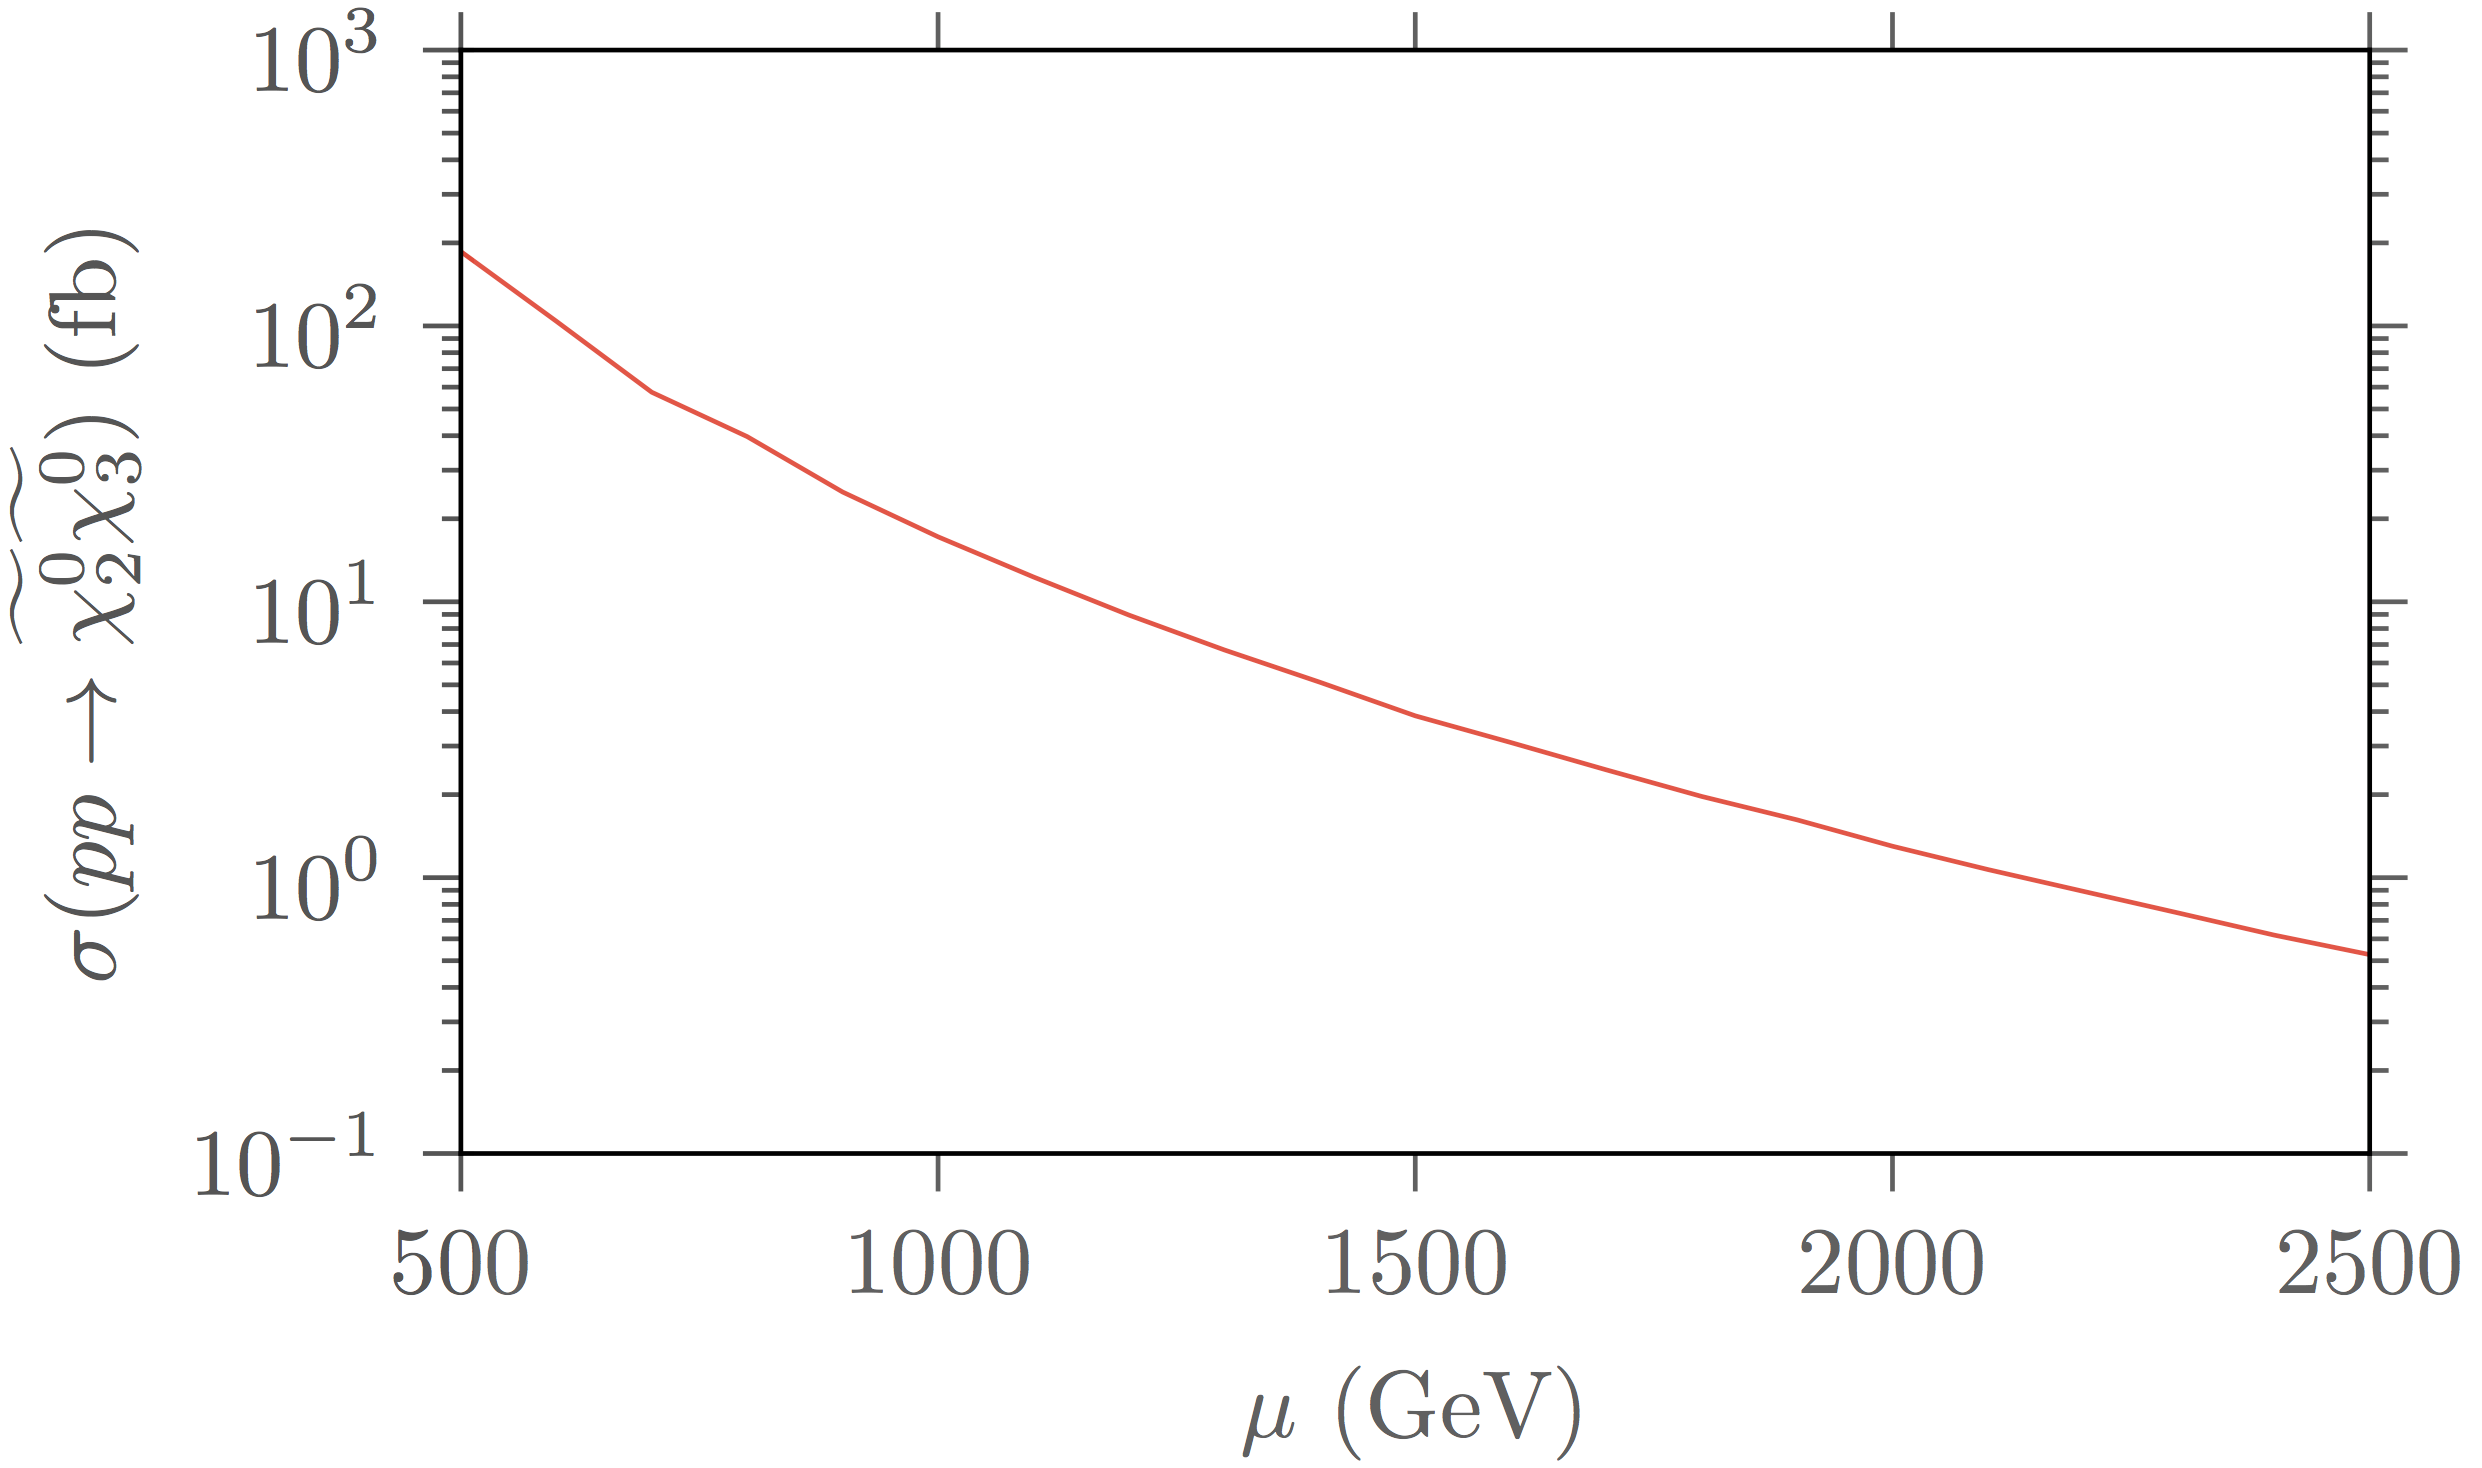
\includegraphics[width=0.49\textwidth]{images/higgsino_production_xsection.png}
  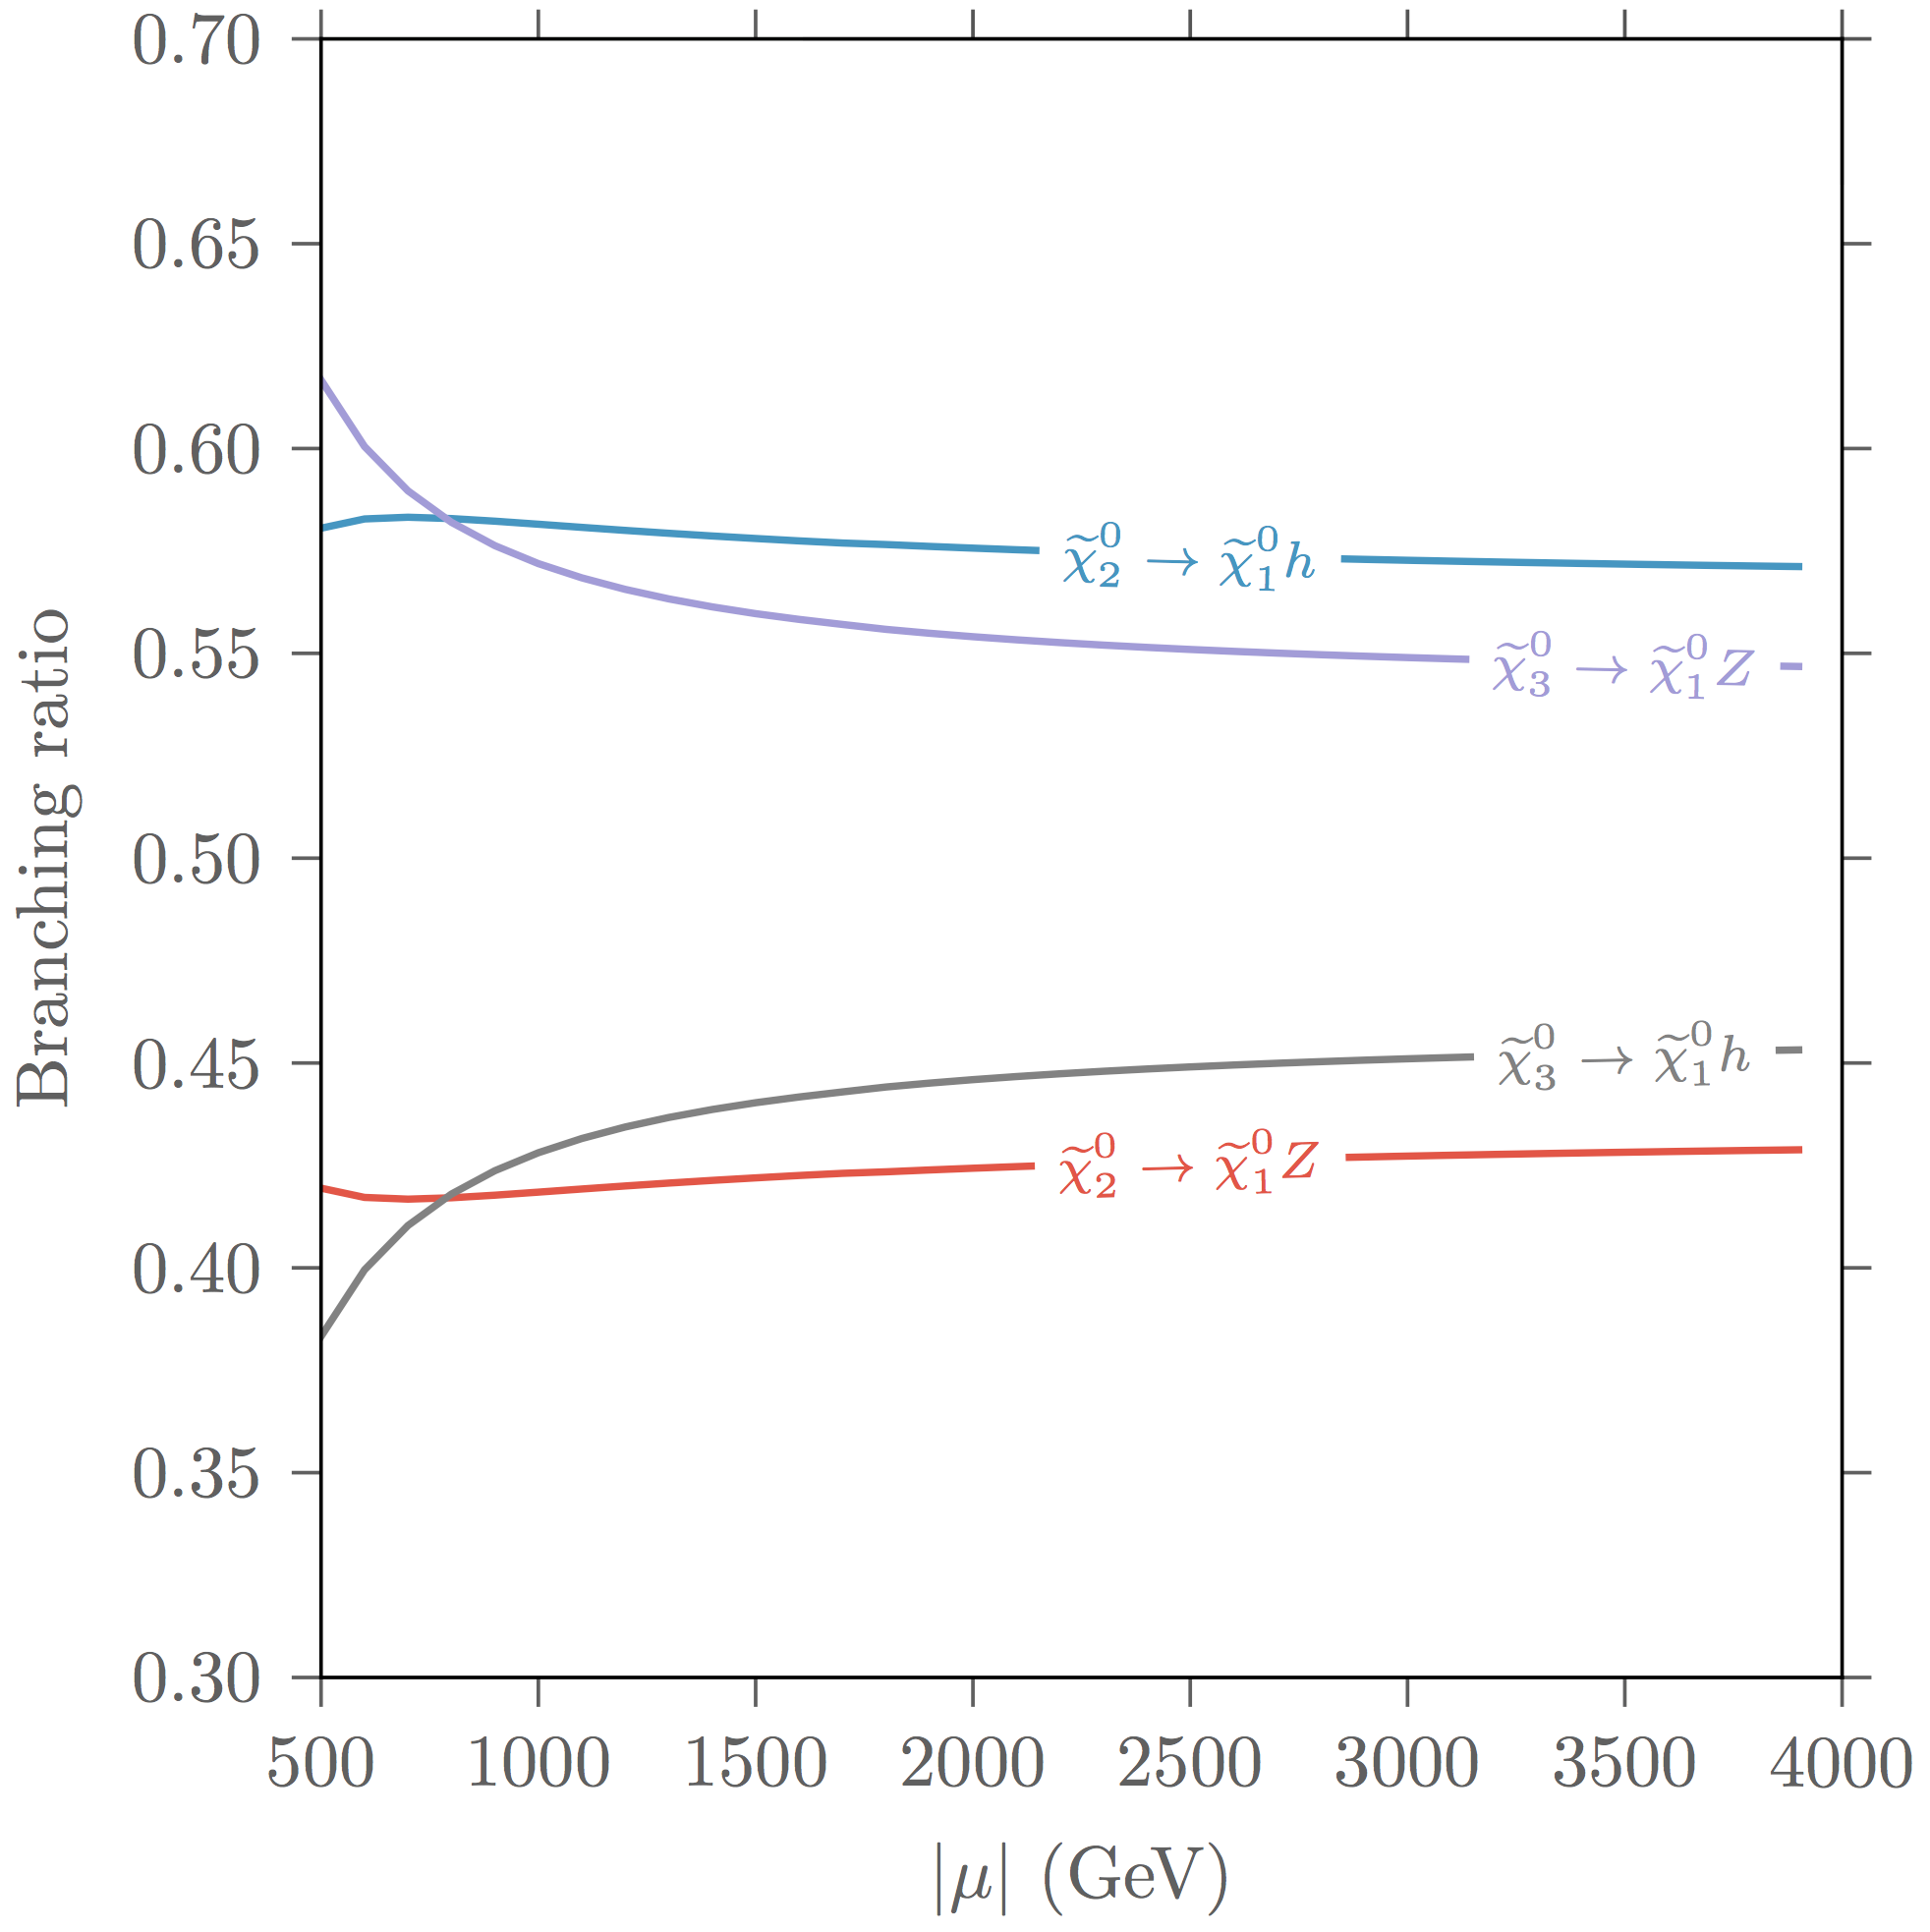
\includegraphics[width=0.49\textwidth]{images/higgsino_br_plot.png}
  \caption{Higgsino pair production cross section, as a function of $|\mu|$. The
  cross-sections are calculated using Prospino2, with $M_1 = 25$ GeV. However, it
  should be noted that the dependence on $M_1$ is very weak.  \Shufang{Could you make the two plot same aspect ratios?}}
  \label{fig:xsection_plot}
\end{figure}

 

Searches for pair produced nearly mass-degenerate Higgsinos  have been performed 
at ATLAS and CMS for various decay  topologies. While the identity of the 
LSP in these searches is a gravitino  instead of a Bino,   the limits are still  relevant, since both  our analysis  and the experimental ones consider that  
the neutral Higgsinos decay to a  neutral SM boson (\emph{h/Z})  and the 
LSP 100\% of the time.  \Shufang{But this is not the same as our Higgsino NLSP and Bino LSP case.}

The most stringent limits are obtained by ATLAS in \cite{Aaboud:2018htj},
where Higgsinos with masses between 130 and 230 GeV and between 290 and 880 
GeV are excluded using a search channel with a final state containing 3+ 
\emph{b}-jets. \Shufang{you mean more than 3 b jets?} The CMS analysis
in \cite{Sirunyan:2017ubx} which uses a combination of channels and final states 
$4b+\slashed{E}_T, 2l + 2j + \slashed{E}_T, 3l/4l + \slashed{E}_T$ and $2\gamma+\slashed{E}_T$ 
to exclude Higgsino-like neutralino masses up to 650-750 GeV, depending on the assumed branching 
fraction of the neutralino decays. Finally, the $4l$ final state has been studied by ATLAS in \cite{Aaboud:2018zeb}
to set a lower bound of 295 GeV on the Higgsino mass  \cite{Aaboud:2018zeb}.
\Shufang{So the only available limit is with gravitino LSP?  Then it does not apply.}
\Shufang{There is no  WZ+MET limit on Higgsinos NLSP?}



%ATLAS 1806.04030, (hh/hZ/ZZ/) --> 4b
% CMS 1801.03957, combination of channels
% 4b + MET, 2l + 2j + MET, >3l + MET, diphoton + MET
% ATLAS, 4 leptons (hh/ZZ/hZ --> 4l)

\begin{comment}
While the majority of the existing searches for supersymmetry focus on gluino
pair production, there are a number of analyses involving electroweak pair
production of charginos and neutralinos as well, which we will attempt to briefly review here.  Searches
involving multiple leptons and missing energy $(2l/3l +\slashed{E}_T)$ in the
final state are described in
\citep{Aaboud:2018sua,Aaboud:2018jiw, ATLAS:2016uwq,Khachatryan:2014qwa,Chatrchyan:2012pka}, assuming a
wino-like NLSP and a bino-like LSP. The best reach is obtained in the $2/3l$
channel by ATLAS with 36.1 fb$^{-1}$ of data, with NLSP masses up to 600 GeV
excluded for massless LSPs \citep{Aaboud:2018sua}.

% AP: These have intermediate sleptons, so I am omitting them.
%Topologies with one or two hadronically-decaying tau leptons and missing energy
%in the final state have been studied in \citep{ATLAS:2016ety,
%Khachatryan:2016trj}, with the greatest reach obtained by ATLAS in
%\citep{ATLAS:2016ety}, using 13 TeV data - they are able to exclude wino-like
%NLSPs up to a mass of 700 GeV for a massless bino-like LSP. 

Searches with a combination of leptons and jets in the final states can be found
in \citep{Aad:2014vma,Khachatryan:2015kxa,Khachatryan:2014mma}. Winos up to 465
GeV are excluded in the $2l + 0/2j$ final states in \citep{Aad:2014vma}. A
compressed mass spectrum is studied in \citep{Khachatryan:2015kxa}, with a mass
difference of about 50 GeV between winos and binos. This study uses the vector
boson fusion channel, with a final state of $2l + 2j + \slashed{E}_T$, and
excludes winos up to a mass of 170 GeV. Of particular interest to us is the
analysis in \citep{Khachatryan:2014mma}, where higgsinos can be excluded up to a
mass of 380 GeV using the $bbll + \slashed{E}_T$ final state, but cannot be
discovered in any region of the relevant parameter space. As we shall see, a 100
TeV collider will enable us to greatly improve upon these limits.
\end{comment}

\section{Analysis Details}\label{sec:analysis}

In this section, we  describe our strategies for both the traditional
cut-and-count analysis, as well as the analysis carried out with boosted
decision trees. 

\subsection{Simulation}\label{simulation}

We simulated parton-level events using \texttt{MadGraph5 v2.3.2.2} and
\texttt{MadEvent} \citep{Alwall:2014hca}, then passed those events to Pythia 6
\citep{Sjostrand:2006za} for showering and hadronization. Finally, we used
\texttt{Delphes 3} \citep{deFavereau:2013fsa} to perform a fast, parametrized
detector simulation, with the detector card devised by the FCC-hh working
group\footnote{\url{https://github.com/HEP-FCC/FCCSW/blob/master/Sim/SimDelphesInterface/data/FCChh_DelphesCard_Baseline_v01.tcl}}.
For the backgrounds, we allowed up to one additional jet in the final state, to
approximate NLO QCD effects, and performed MLM matching with the \texttt{xqcut}
parameter set to 40 GeV. The Higgsino pair production cross sections were
calculated using \texttt{Prospino2} \citep{Beenakker:1999xh}. \Shufang{tree level or NLO or what?}  To decouple the
Wino, we set its mass parameter $M_2$ to 3 TeV.  \Shufang{5 TeV was used for another calculation earlier.  Be consistent here.}

Since we expect our signal process to have a dilepton resonance from an on-shell
$Z$ boson, we restricted the phase space for event generation for backgrounds to
the region where the invariant mass of dilepton pairs lies between 80 and 100
GeV. Additionally, the Bino dark matter that escapes the detector would result
in a large amount of missing transverse energy ($\met$), so we required
a minimum $\met$ of 100 GeV at the parton level for the backgrounds as
well. 

At the detector simulation level, we relaxed the lepton isolation criterion in the
\texttt{Delphes} detector card from $\Delta R_{min}$ from 0.4 to 0.05. This is
motivated by the fact that due to the large mass difference between the Higgsino
NLSP and the Bino LSP in our search channel, the intermediate $Z$ bosons will be
highly boosted, and the leptons to which they decay will be highly collimated.
The value of 0.05 is consistent with what is suggested in previous 100 TeV
studies (\citep{Acharya:2014pua,Gori:2014oua,Bramante:2014tba}) and will allow
for easier comparison between different search strategies.


\subsection{Analysis using cut-and-count}
\label{event-selection}

For the cut-and-count analysis, we implemented successive one-dimensional cuts
on the variables listed below, using the MadAnalysis 5 package
\citep{Conte:2012fm}.

\begin{enumerate}
  \tightlist
  \item \emph{Trigger}: Events were selected if they had at least one lepton
    with $p_{T}^\ell >$ 100 GeV.  \Shufang{This is quite a high trigger level cut.  Is the 100 TeV lepton trigger need such a high pT? or it is a lower pT trigger, with a 100 GeV advanced cut to suppress the bg?}

  \item \emph{Identification:}

    \begin{itemize}
      \item Events contain exactly two leptons of the same flavor
        and with opposite signs (\textsc{sfos}), with $p_{T}^\ell >$ 15 GeV and
        $\vert\eta^\ell\vert <$ 2.5.
      \item Events contain at least two \emph{b}-tagged jets with
        $p_{T}^b > 30$ GeV and $\vert\eta^b\vert <$ 2.5.
    \end{itemize}

  \item \emph{Invariant mass of Z-candidate:}  $85\ {\rm GeV}<m_{\ell^{+}\ell^{-}}<95\ {\rm GeV}$.

  \item \emph{Invariant mass of h-candidate:} $75\ {\rm GeV}<m_{bb}<150\ {\rm GeV}$ for two leaving $b$-jets.

  \item \emph{Missing Tranverse Energy:}  $\met> 400$ GeV.

  \item \emph{Razor variables}:  Two razor variables are used in our analyses: 
\begin{eqnarray}
M_R &=& \sqrt{(E_Z+E_h)^2 - (p_Z^z + p_h^z)^2},\\ M_T^R &=& \sqrt{\frac{1}{2}\left[\slashed{E}_T(|\vec{p}_{ZT}|+|\vec{p}_{hT}|)^2 - \vec{\slashed{E}}_T\cdot(\vec{p}_{ZT}+\vec{p}_{hT})\right]},
\end{eqnarray} 
 for$E_{Z,h}$ and $p_{Z,h}$ being the reconstructed energy and momentum for $Z$ and $h$.
\Shufang{Check the formula.  Unit is not correct.}
    Representative kinematic
  distributions of these variables for signal events of a 1 TeV Higgsino and a 25 GeV Bino, as well as $tt$ and $tbW$ backgrounds are
  shown in Fig.~\ref{fig:razor_histos}, after the trigger, identification, and
  $\slashed{E}_{T}$ cuts. The
  distribution for the \emph{bbWW} background is not shown, since it is negligible in
  comparison to the others.   We can see that the distribution of $M_R$ is peaked
  around 1 TeV for the signal, which consistent with what we would expect, since
  it corresponds to the mass difference between the NLSP and LSP.  For this mass combination, requiring $M_R >$ 800
  GeV and $M_T^R >$ 400 GeV yields the greatest significance.

\end{enumerate}

\begin{figure}[h]
\centering
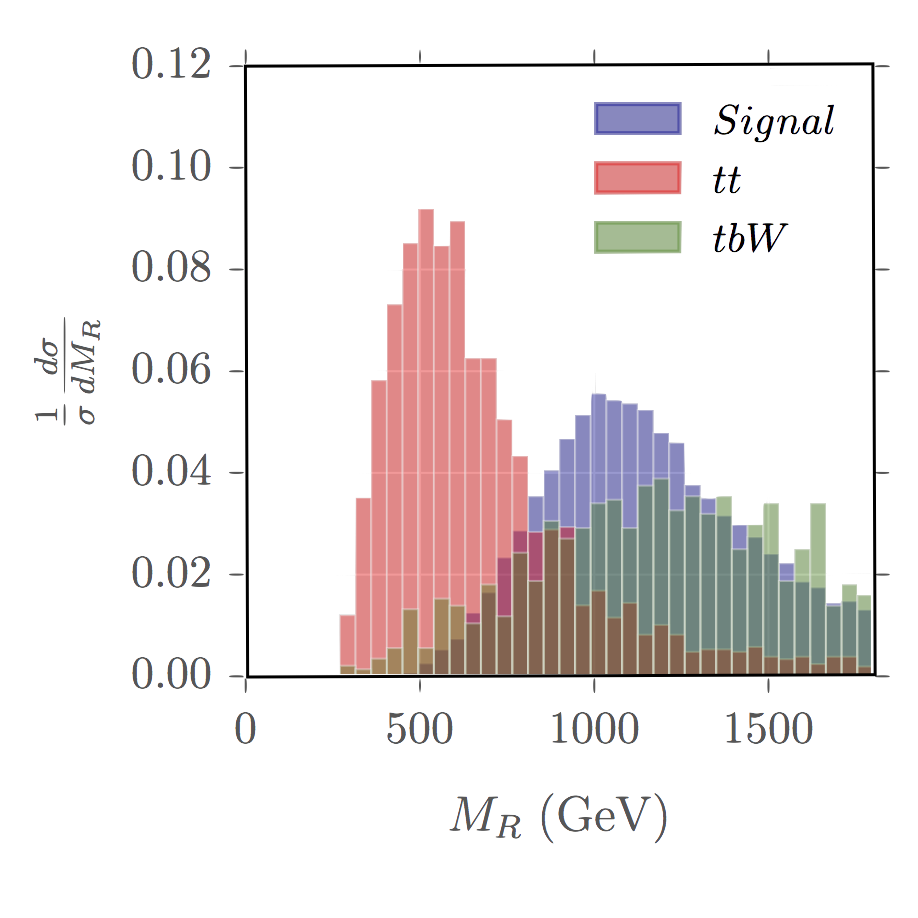
\includegraphics[trim = {0.3cm 0.6cm 0.1cm 0}, clip, width=0.496\textwidth]{images/mR_copy.png}
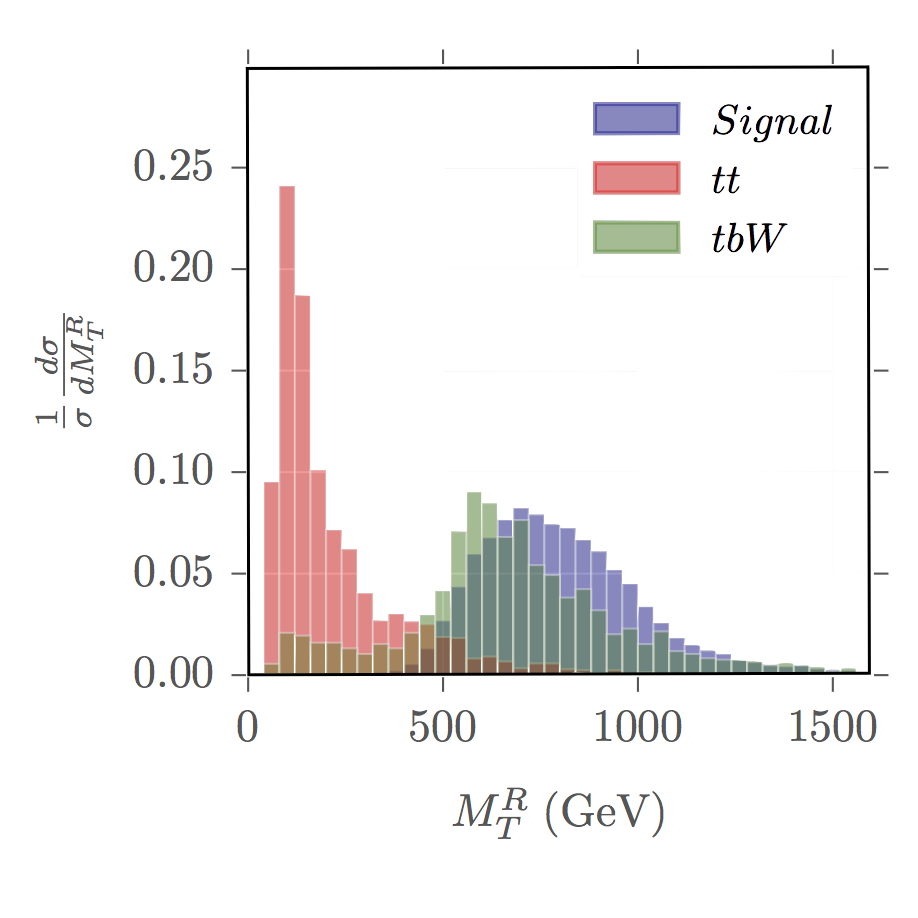
\includegraphics[trim = {0.3cm 0.6cm 0.1cm 0}, clip, width=0.496\textwidth]{images/mTR_copy.png}
\caption{Normalized distributions of the razor kinematical variables $M_R$
  (left) and $M_T^R$ (right) for signal process with a 1 TeV Higgsino NLSP and 25 GeV Bino LSP,  as well as the dominant $tt$ and $tbW$ backgrounds,
  after the trigger, identification, and $\slashed{E}_{T}$ cuts.}
\label{fig:razor_histos}
\end{figure}

\begin{table}[h]
  \centering
  \begin{tabular}{lrrrrrrr}
\toprule
{} &  $\sigma_\text{\emph{signal}}$ &  $\sigma_{t\overline{t}}$ &  $\sigma_\text{\emph{tbW}}$ &  $\sigma_\text{\emph{bbWW}}$ &  $\sigma_\text{\emph{BG (total)}}$ &   $S/B$ &  $S/\sqrt{B}$ \\
\midrule
Original            & 0.37 & 35,998 & 4,176 & 7.8     & 40,182 & 9.1$\times$ 10$^{-6}$ & 0.10 \\
Trigger             & 0.31 & 5,321  & 1,058 & 2.5     & 6,382  & 4.9$\times$ 10$^{-5}$ & 0.21 \\
\textsc{sfos} leptons        & 0.25 & 1,774  & 360   & 0.88    & 2,135  & 1.2$\times$ 10$^{-4}$ & 0.30 \\
2 $b$ jets          & 0.04 & 290    & 62    & 0.09    & 352    & 1.3$\times$ 10$^{-4}$ & 0.13 \\
$\slashed{E}_T >$ 400         & 0.03 & 5.3    & 6.8   & 0.007   & 12     & 0.003               & 0.49 \\
$m_{ll} \in$ [85, 95]  & 0.03 & 2.1    & 3.3   & 0.004   & 5.3    & 0.005               & 0.62 \\
$m_{bb}\in$ [75,150] & 0.02 & 0.59   & 0.30  & 8.2$\times$ 10$^{-4}$ & 0.90   & 0.02                & 1.3 \\
$M_{R} >$ 800       & 0.02 & 0.03   & 0.20  & 3.3$\times$ 10$^{-4}$ & 0.23   & 0.09                & 2.2 \\
$M_{T}^{R} >$ 400   & 0.02 & 0.008  & 0.18  & 1.9$\times$ 10$^{-4}$ & 0.19   & 0.10                & 2.4 \\
\bottomrule
\end{tabular}

  \caption{Representative cut flow table for the benchmark point $|\mu|=1$ TeV,
    $M_1 = 25$ GeV, for a traditional cut-and-count analysis. All cross sections
    are given in femtobarns, and the units for the missing energy, invariant
    mass, and razor variable cuts are GeV. The significance, $S/\sqrt{B}$, is
    calculated for an integrated luminosity of 3 ab$^{-1}$.    }
\label{tab:cc_cutflowtable}
\end{table}

Table \ref{tab:cc_cutflowtable} shows the cut efficiencies for a representative
signal benchmark point with a $|\mu| =$ 1 TeV and $M_1$ = 25 GeV.   The
cross-sections of the backgrounds are averages \Shufang{What do you mean by average?}  of the cross-sections output by
MadEvent after performing the MLM matching procedure. Their small size reflects
the $m_{\ell\ell}$ and $\slashed{E}_T$ cuts we imposed at the parton level. For all
the benchmark points, we require a minimum of 5 signal events left over after
cuts. We can see that, after applying our cuts, $tt$ and $tbW$ remain as the
dominant backgrounds. The values of the razor variable cuts were chosen to
maximize the significance, $S/\sqrt{B}$ (calculated for an integrated luminosity
of 3000 fb$^{-1}$), shown in the last column.  \Shufang{For the reach plot, does razor variable cut value changes for each grid point?}

\subsection{Analysis using gradient boosted decision trees}\label{subsec:bdt}

For each signal mass combination and each background process, we preselected
events that passed the lepton trigger, contained two SFOS leptons and two
$b$-tagged jets, and calculated a number of kinematic variables for each event. We then
placed these kinematic variables in an array, with each row corresponding to an event, and
the columns corresponding to the kinematic variables. A mixture of low-level and high level
kinematic variables was shown to have the greatest effectiveness. The kinematic variables chosen were
$m_{\ell\ell}$, $m_{bb}$, $M_R$, $M_T^R$, $\slashed{E}_T,$ the total hadronic
transverse energy $THT$, \Shufang{THT?} and transverse momenta of individual final state
leptons and $b$-quarks: $p_T^{\ell_1}$, $p_T^{\ell_2}$, $p_T^{b_1}$, and $p_T^{b_2}$. We
then divided the events into training and test sets, with the training set
comprising 75\% of signal events and 30\% of background events. \Shufang{You mean 70\% of all signal event generated? } We used the
\texttt{scikit-learn} package  \citep{Pedregosa2011} to implement our analysis.
{\it A boosted decision tree classifier was trained with 1000 weak learners and a
learning rate of 0.025. } \Shufang{We probably don't need this details.}  After the classifier is trained, we use it to assign
scores to individual events. A more negative score indicates a more
background-like event, and a more positive score denotes a more signal-like
event. After the scores have been assigned to the events in the test sets, we
can use this score just as we would a regular kinematical variable, that is, we
apply a cut that selects events with a minimum of this score. The value of the
cut is chosen to maximize the significance for each signal benchmark point. The
distribution of scores for the specific benchmark point ($|\mu|$ = 1 TeV, $M_1$
= 25 GeV) is shown in figure \ref{fig:bdt_response}. We observe that there is an
appreciable separation between the signal and background distributions.

\begin{figure}[h]
\centering
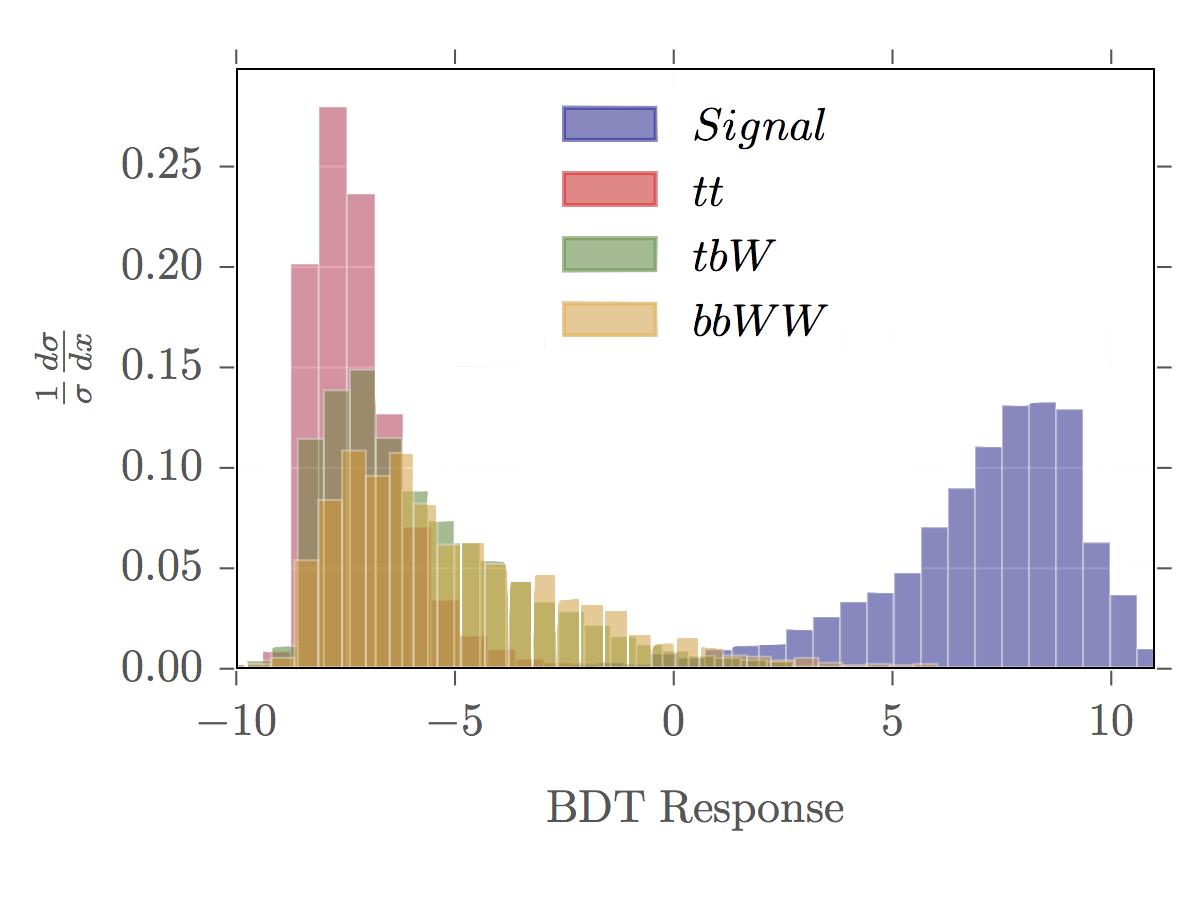
\includegraphics[trim = {0 0.5cm 0 0},clip]{images/bdt_response_png}
\caption{Distribution of the decision function of the gradient boosted decision
tree classifier algorithm for signal ($|\mu| = 1$ TeV $M_1 = 25$ and
backgrounds. }
\label{fig:bdt_response}
\end{figure}

\begin{table}[h]
  \centering
  \begin{tabular}{lrrrrrrr}
\toprule
{} &  $\sigma_\text{\emph{signal}}$ &  $\sigma_{t\overline{t}}$ &  $\sigma_\text{\emph{tbW}}$
   &  $\sigma_\text{\emph{bbWW}}$ &  $\sigma_\text{\emph{background (total)}}$ &   $S/B$ &  $S/\sqrt{B}$ \\
\midrule
Original           &               0.37 &          35,998 &           4,176 &              7.8 &             40,182 & 9.1e-06 &          0.10 \\
Preselection &               0.04 &             290 &              62 &             0.09 &                352 & 1.3e-04 &          0.13 \\
\textsc{bdt} response $> 5.1$      &               0.04 &            0.02 &            0.04 &          4.8e-04 &               0.06 &    0.63 &           8.4 \\
\bottomrule
\end{tabular}

  \caption{Representative cut flow table for the same benchmark point and
    integrated luminosity as in table \ref{tab:cc_cutflowtable}, but using a
    boosted decision tree (BDT) analysis instead. The preselection is equivalent
    to the trigger and identification cuts listed in table
    \ref{tab:cc_cutflowtable}. As before, all the cross sections are in
  fb.  }
\label{tab:bdt_cutflowtable}
\end{table}

Table \ref{tab:bdt_cutflowtable} shows the cut efficiences for the same
representative benchmark point as in table \ref{tab:cc_cutflowtable}, but this
time for a boosted decision tree analysis. We observe that the statistical
significance we can achieve goes up from 2.4 to 8.4, a roughly four-fold
increase.  \Shufang{Do we still require 5 signal events minimum here?}

For certain values of the
cuts on kinematical variables or the score of the classifier, no events survived
for one or more of the background components. To guard against overly optimistic
estimates of the significance $S/\sqrt{B}$, we set a lower bound of 3 for the
number of MC events after cuts for each background component, corresponding to
the 95\% confidence interval for a Poisson distribution. 


\begin{figure}[h]
\centering
%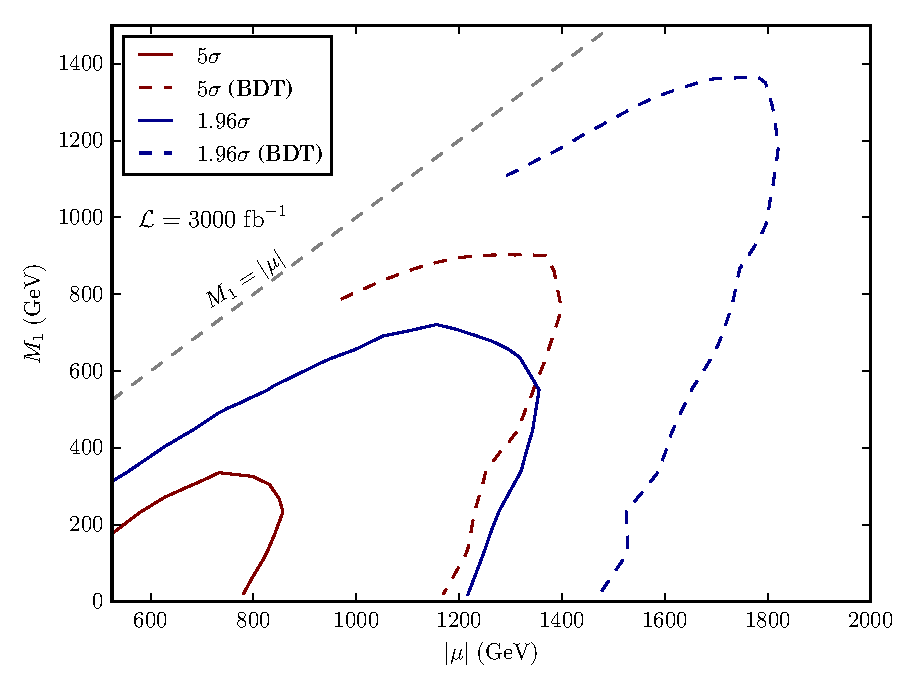
\includegraphics[width=0.6\textwidth]{images/combined.pdf}
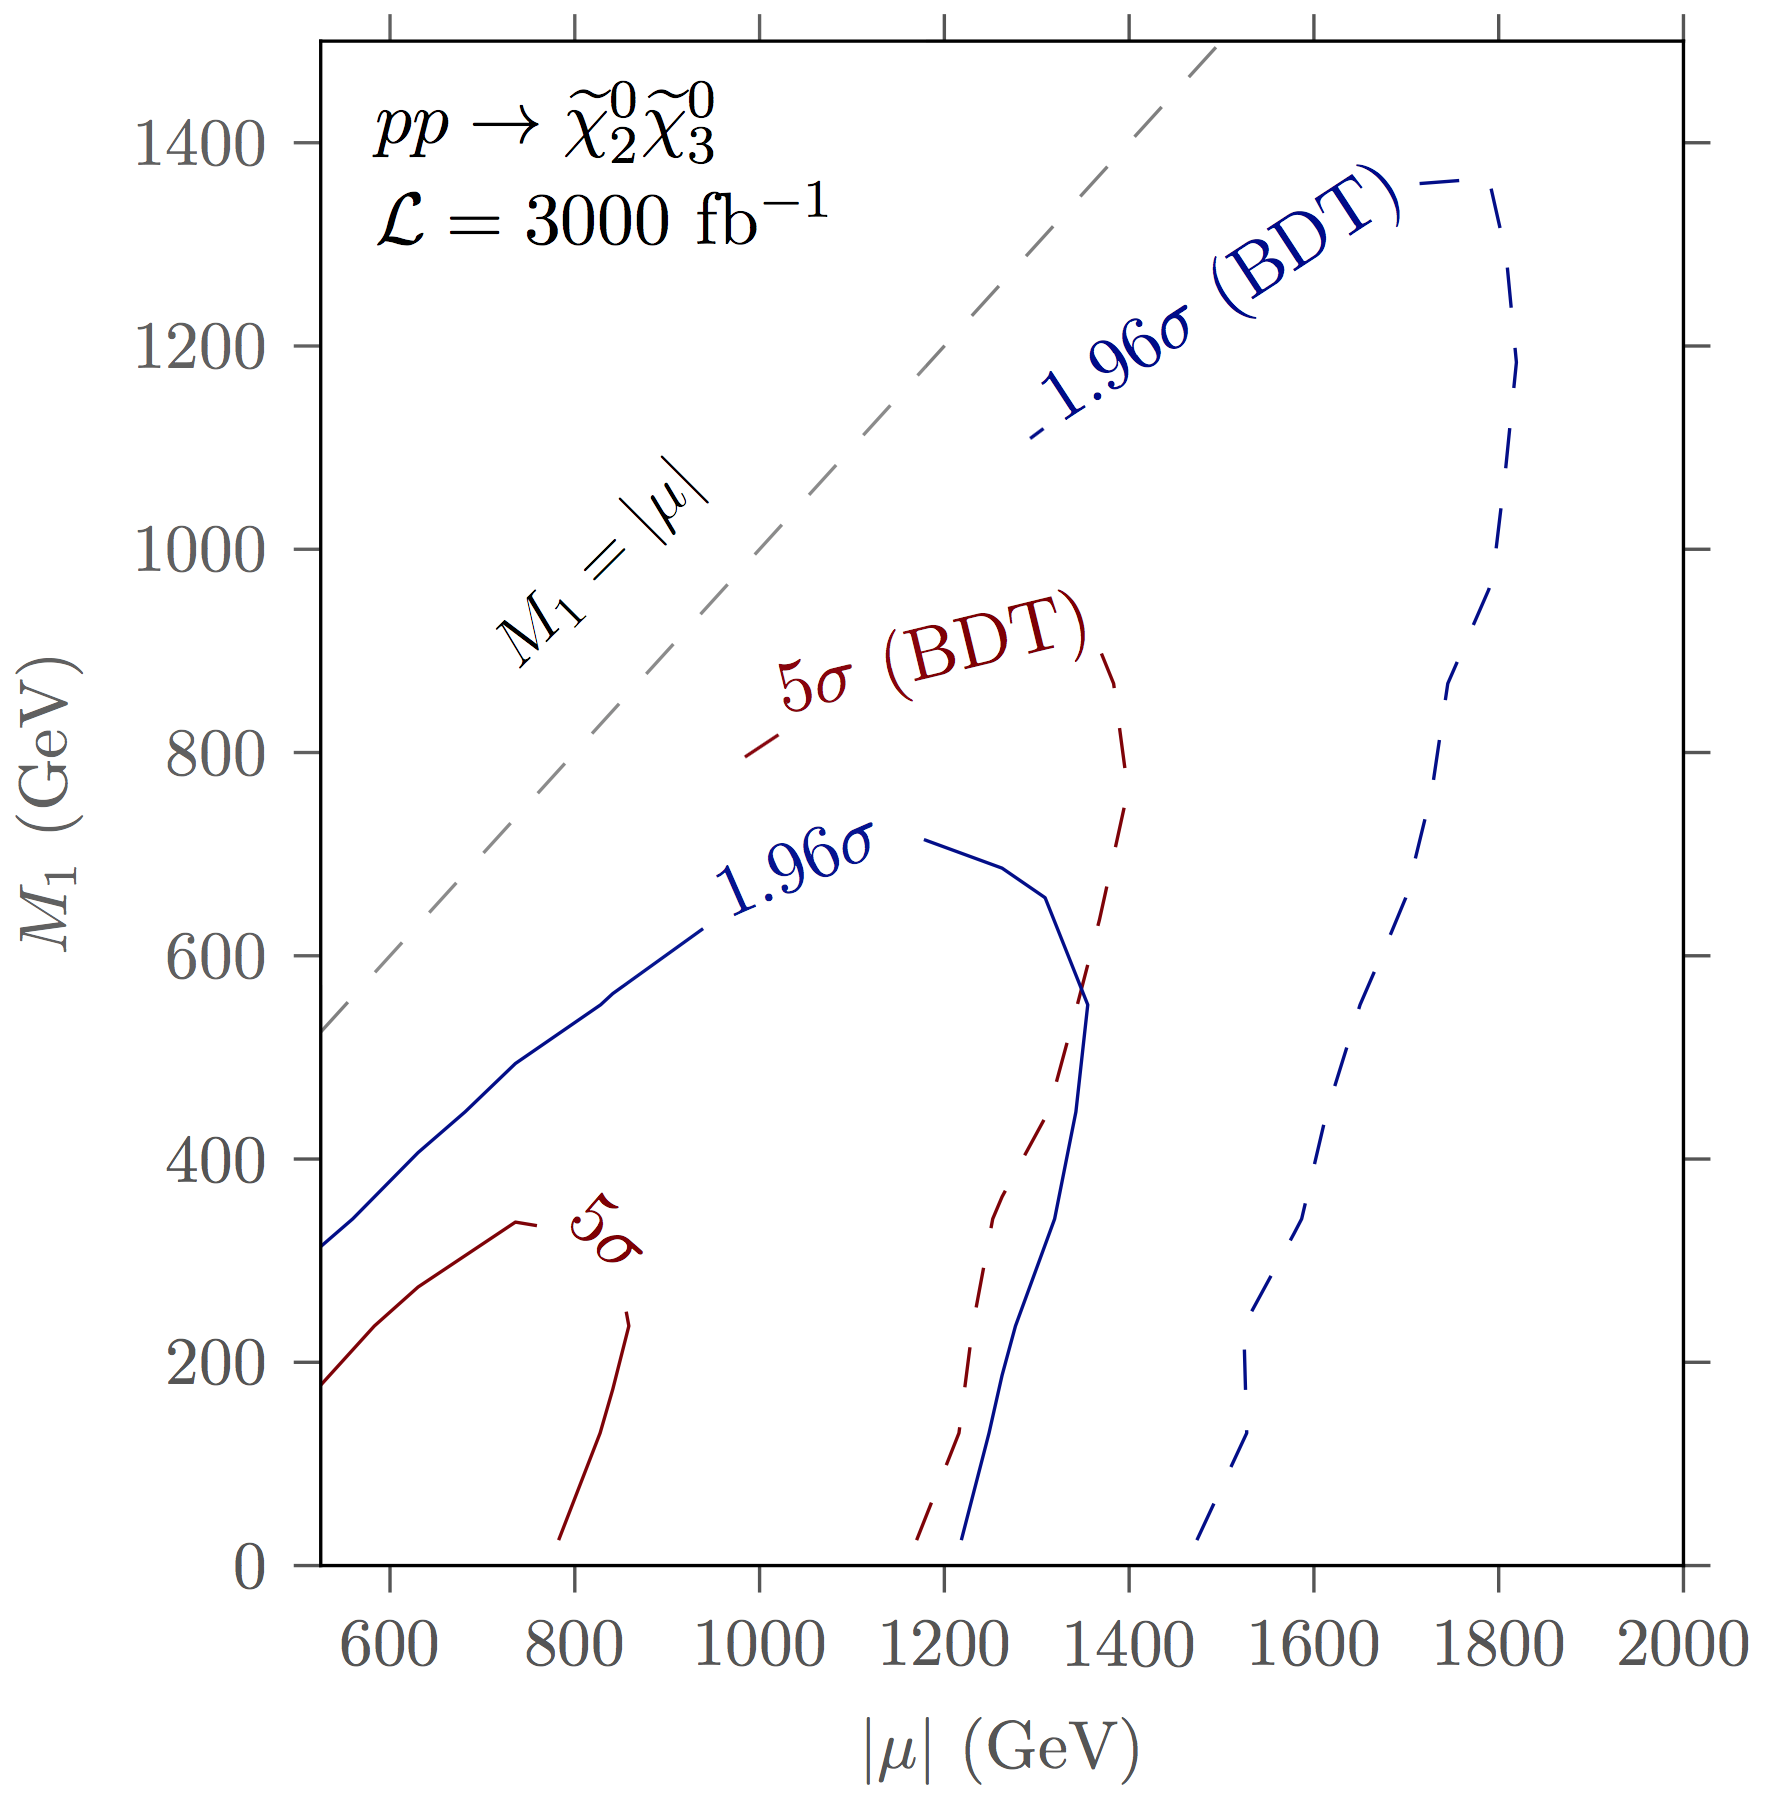
\includegraphics[width=0.6\textwidth]{images/dm_100_TeV_contours.png}

\caption{ Discovery (red) and exclusion (blue) contours for the traditional
  cut-and-count analysis (solid) and boosted decision tree analysis (dashed),
  for 100 TeV $pp$ collider with an integrated luminosity of 3000 fb$^{-1}$. \Shufang{Shall we show the lepton search result in this figure for comparison?} }

\label{fig:contours}
\end{figure}

\section{Discovery and exclusion limits}
\label{sec:results}

Fig.~\ref{fig:contours} shows the expected reach in parameter space for
95\% C.L. exclusion and 5$\sigma$ discovery in the parameter space of $|\mu|$ vs. $M_1$ for 100 TeV $pp$ collider with an integrated luminosity of 3000 fb$^{-1}$. The cut-and-count strategy is able to discover
Higgsinos up to 750 GeV  and exclude them up to 1.3 TeV. \Shufang{How do you read out the numbers?}  The boosted decision
tree analysis, improves this reach - it is able to discover Higgsinos up to 1.3
TeV, and exclude them up to 1.8 TeV in favorable points in parameter space.
Similarly, Binos can be discovered up to 300 GeV and excluded up to 800 GeV with
the rectangular cut analysis, and the BDT analysis can discover them up to about
900 GeV and exclude them up to 1.3 TeV. Table \ref{tab:summary} contains a
summary of these results. Since the background left after cut is relatively low, We do not include systematic errors in these
estimates.  

This improvement is substantial, but perhaps not spectacular. However, it should
be kept in mind that this is probably a conservative estimate. Since we reserve
30\% of the data for training purposes, and impose the condition that the
minimum number of MC events after cuts for the backgrounds must be 3 (see note
at the end of subsection \ref{subsec:bdt}), the true rate of background
rejection by the classifier is likely underestimated, and the expected
significance from the BDT analysis will improve. This extrapolation is
qualitatively supported by the high degree of separation between signal and
backgrounds seen in Fig.~\ref{fig:bdt_response}, and the fact that a larger
fraction of the signal events are preserved with the BDT approach compared to
the rectangular cut approach, as can be seen in Tables \ref{tab:cc_cutflowtable}
and \ref{tab:bdt_cutflowtable}.  

In regions with large mass differences between the LSP and NLSP, the reach is
not as good, since the intermediate SM Higgs boson will be highly boosted, and
thus decay into a highly collimated pair of $b$-jets. The extent to which this
affects our results can be estimated from table \ref{tab:cc_cutflowtable}. We
see that requiring two $b$-tagged jets reduces our signal cross-section by
roughly 87\%. This is far more than the 28\% reduction that one might naively
expect as a result of applying the $b$-tagging efficiency of about 85\%
specified in our \texttt{Delphes} card.  \Shufang{How do you get the 28\% number? }

\begin{table}[h]
\centering
\begin{tabular}{l|rr}
\toprule
Analysis type & 5$\sigma$ (discovery)& 1.96$\sigma$ (exclusion)\\
\midrule
Rectangular cuts & (0.75, 0.30) & (1.3, 0.8)\\
BDT Analysis & (1.3, 0.90) & (1.8, 1.3)\\
\bottomrule
\end{tabular}
\caption{Discovery reaches and expected exclusion limits (in TeV) for the
parameters $(|\mu|,M_1)$ for the rectangular cuts and BDT analyses. \Shufang{Probably don't need this table.} }
\label{tab:summary}
\end{table}

\section{Conclusion}\label{sec:conclusion}

In this paper, we examined the discovery potential for a 100 TeV $pp$ collider For 
pair-produced heavy Higgsinos with Bino LSP, via 
intermediate $Z$ and $h$ bosons that decay to a pair of leptons and $b$ quarks
respectively.   

We pursued two analysis strategies. One was the traditional cut-and-count methos , including razor variables
that are sensitive to the mass difference between the LSP and the NLSP. The
other strategy was to use a boosted decision tree classifier trained with a
number of low- and high-level kinematic variables, including razor variables. We expected
that the machine learning approach would be able to more efficiently determine
the optimal decision boundary between signal and background events in feature
space than the traditional   cut-and-count method.

Overall, we find that the reach of our analysis strategy is a significant
improvement over that of the LHC.  \Shufang{Did we mention the LHC reach?}  We found that the rectangular cut strategy has
the potential to discover Higgsino LSPs up to a mass of 750 GeV, and exclude
them up to a mass of 1.3 TeV. As expected, the boosted decision tree classifier
performs better, with the ability to discover Higgsino NLSPs up to 1.3 TeV and
exclude them up to a mass of 1.8 TeV. With the BDT analysis, Bino dark matter
candidates can be discovered up to 900 GeV, and excluded up to 1.3 TeV. In the
process, we highlighted the importance of generating enough Monte Carlo events
to estimate the huge backgrounds at a 100 TeV $pp$ collider. 

Additionally, we found that the reach for both strategies is considerably
reduced when the difference $ |\mu|-M_1$ is high, since it results in a highly
boosted $h$ that decays to a collimated pair of $b$'s that will most likely be
identified as a single jet. This is not an insurmountable difficulty - there are
ways to deal with collimated jets, although they are beyond the scope of this
work. This issue does, however, highlight the necessity of improving isolation
performance at a 100 TeV $pp$ machine, where large mass hierarchies can result in
highly boosted/collimated decay products. For a review of currently used methods
to determine jet substructure, see \citep{Shelton:2013an}. In the future,
machine learning techniques might be profitably applied to this area as well -
for a review of developments along this line, see \citep{Schwartzman:2016jqu}. 

The collimation of the $b$-jets, along with the fact that we take into account
detector effects using Delphes, result in a lower reach in the high $|\mu|$, low
$M_1$ region than the multilepton analysis in \citep{Gori:2014oua}, which is
able to exclude Higgsinos up to a mass of 2.9 TeV for massless binos. The reach
of our analysis is slightly higher in the region where the difference between
$|\mu|$ and $M_1$ is smaller. This is consistent with our usage of the razor
variable $M_R$, which is sensitive to the mass difference between the parent
Higgsino and daughter Bino.

A 100 TeV $pp$ collider represents an excellent opportunity to discover
physics beyond the Standard Model. The extremely high energies and luminosities
involved will present new challenges for particle physicists, and it is likely
that machine learning will play an important part in facing them. 
  
\acknowledgments

We would like to thank Matt Leone and Ken Johns for helpful discussions.  The
research activities of AP and SS were supported in part by the Department of
Energy under Grant DE-FG02-13ER41976 / de-sc0009913;. An allocation of computer
time from the UA Research Computing High Performance Computing (HPC) and High
Throughput Computing (HTC) at the University of Arizona is gratefully
acknowledged.

\bibliography{references}

\end{document}
